% Docummentclass 
\documentclass[a4paper, oneside, titlepage]{report}
% Packages
\usepackage{amsmath}
\usepackage{complexity}
\usepackage[T1]{fontenc}
\usepackage[utf8]{inputenc}
\usepackage[pdftex]{graphicx} %%Graphics in pdfLaTeX
\usepackage{a4wide} %%Smaller margins, more text per page.
\usepackage{longtable} %%For tables that exceed a page width
\usepackage{pdflscape} %%Adds PDF sup­port to the land­scape en­vi­ron­ment of pack­age
\usepackage{caption} %%Pro­vides many ways to cus­tomise the cap­tions in float­ing en­vi­ron­ments like fig­ure and ta­ble
\usepackage{float} %%Im­proves the in­ter­face for defin­ing float­ing ob­jects such as fig­ures and ta­bles
\usepackage[tablegrid,nochapter]{vhistory} %%Vhis­tory sim­pli­fies the cre­ation of a his­tory of ver­sions of a doc­u­ment
\usepackage[nottoc]{tocbibind} %%Au­to­mat­i­cally adds the bib­li­og­ra­phy and/or the in­dex and/or the con­tents, etc., to the Ta­ble of Con­tents list­ing
\usepackage[toc,page]{appendix} %%The ap­pendix pack­age pro­vides var­i­ous ways of for­mat­ting the ti­tles of ap­pen­dices
\usepackage{pdfpages} %%This pack­age sim­pli­fies the in­clu­sion of ex­ter­nal multi-page PDF doc­u­ments in LATEX doc­u­ments
\usepackage[rightcaption]{sidecap} %%De­fines en­vi­ron­ments called SC­fig­ure and SCtable (anal­o­gous to fig­ure and ta­ble) to type­set cap­tions side­ways
\usepackage{cite} %%The pack­age sup­ports com­pressed, sorted lists of nu­mer­i­cal ci­ta­tions, and also deals with var­i­ous punc­tu­a­tion and other is­sues of rep­re­sen­ta­tion, in­clud­ing com­pre­hen­sive man­age­ment of break points
\usepackage[]{acronym} %%This pack­age en­sures that all acronyms used in the text are spelled out in full at least once. It also pro­vides an en­vi­ron­ment to build a list of acronyms used
\usepackage[pdftex,scale={.8,.8}]{geometry} %%The pack­age pro­vides an easy and flex­i­ble user in­ter­face to cus­tomize page lay­out, im­ple­ment­ing auto-cen­ter­ing and auto-bal­anc­ing mech­a­nisms so that the users have only to give the least de­scrip­tion for the page lay­out. For ex­am­ple, if you want to set each mar­gin 2cm with­out header space, what you need is just \usep­a­ck­age[mar­gin=2cm,no­head]{ge­om­e­try}.
\usepackage{layout} %%The pack­age de­fines a com­mand \lay­out, which will show a sum­mary of the lay­out of the cur­rent doc­u­ment
\usepackage{subfigure} %%Pro­vides sup­port for the ma­nip­u­la­tion and ref­er­ence of small or ‘sub’ fig­ures and ta­bles within a sin­gle fig­ure or ta­ble en­vi­ron­ment.
\usepackage[toc]{glossaries} %%The glos­saries pack­age sup­ports acronyms and mul­ti­ple glos­saries, and has pro­vi­sion for op­er­a­tion in sev­eral lan­guages (us­ing the fa­cil­i­ties of ei­ther ba­bel or poly­glos­sia).
\usepackage[left,pagewise,modulo]{lineno} %%Adds line num­bers to se­lected para­graphs with ref­er­ence pos­si­ble through the LATEX \ref and \pageref cross ref­er­ence mech­a­nism
\usepackage[pdftex,colorlinks=false,hidelinks,pdfstartview=FitV]{hyperref}%%The hy­per­ref pack­age is used to han­dle cross-ref­er­enc­ing com­mands in LATEX to pro­duce hy­per­text links in the doc­u­ment. 
\usepackage{metainfo}
\usepackage[pagestyles,raggedright]{titlesec}
\usepackage{etoolbox}
\usepackage{%
	array, %%An ex­tended im­ple­men­ta­tion of the ar­ray and tab­u­lar en­vi­ron­ments which ex­tends the op­tions for col­umn for­mats, and pro­vides "pro­grammable" for­mat spec­i­fi­ca­tions
	booktabs, %%The pack­age en­hances the qual­ity of ta­bles in LATEX, pro­vid­ing ex­tra com­mands as well as be­hind-the-scenes op­ti­mi­sa­tion
	dcolumn, %%
	rotating,
	shortvrb,
	units,
	url,
	lastpage,
	longtable,
	lscape,
	qtree,
	skmath,	
}
\usepackage[portuguese]{babel}
\usepackage{booktabs}
\usepackage{array}




\setlength{\parindent}{0pt} %%No indentation at the beginning of paragraphs
\setlength{\parskip}{.5\baselineskip} %%Space between paragraph


% Metadata
% % Metadaten des Dokumentes

\def\Company{Universidade de Taubaté}
\def\Institute{\textit{Universidade de Taubaté, UNITAU}}
\def\Course{\textit{Engenharia de Computação}}
\def\Module{\textit{Automação}}
\def\Docent{\textit{Prof. Patricia}}
\def\Assistant{\textit{}}

\def\BoldTitle{Avaliação Principal }
\def\Subtitle{Projeto de Automação}
\def\Authors{ Cauã dos Santos\\Mateus Ryu Hashimoto \\ Miguel de Paulo \\ Pedro Nassif \\ Thiago \\ Leonardo }
\def\Shortname{}

\title{
\includegraphics[height=5cm]{images/logo.png} \\ \textbf{\BoldTitle}\\\Subtitle}
\author{\Authors \\ \\ \\ \Institute\\ \Course\\ \Module\\ \Docent\\ \Assistant}
\date{Taubaté, 20 Outubro 2025}

%%%%%%%%%%%%%%%%%%%%%%%%%%%%%%%%%%%%%%%%%%%%%%%%%%%%%%%%%%%%%%%%%%%%%%%%%%%%%%%%%
%% Creation of pdf information
%%%%%%%%%%%%%%%%%%%%%%%%%%%%%%%%%%%%%%%%%%%%%%%%%%%%%%%%%%%%%%%%%%%%%%%%%%%%%%%%%
\hypersetup{pdfinfo={
		Title={\BoldTitle: \Subtitle},
		Author={TR},
		Subject={Report}
	}}


% Frontpage
\AtBeginDocument{
  \maketitle
  \thispagestyle{empty}
}

%%%%%%%%%%%%%%%%%%%%%%%%%%%%%%%%%%%%%%%%%%%%%%%%%%%%%%%%%%%%%%%%%%%%%%%%%%%%%%%%%
%% Creation of the header
%%%%%%%%%%%%%%%%%%%%%%%%%%%%%%%%%%%%%%%%%%%%%%%%%%%%%%%%%%%%%%%%%%%%%%%%%%%%%%%%%
\patchcmd{\chapter}{plain}{short}{}{} %$ <-- the header on chapter 1
%%%%%%%%%%%%%%%%%%%%%%%%%%%%%%%%%%%%%%%%%%%%%%%%%%%%%%%%%%%%%%%%%%%%%%%%%%%%%%%%%
%% Creation of page-styles
%%%%%%%%%%%%%%%%%%%%%%%%%%%%%%%%%%%%%%%%%%%%%%%%%%%%%%%%%%%%%%%%%%%%%%%%%%%%%%%%%
\newpagestyle{long}{%
	\sethead[\thepage][][\chaptername\ \thechapter:\ \chaptertitle]{\chaptername\ \thechapter:\ \chaptertitle}{}{\thepage}
	\headrule
}

\newpagestyle{short}{%
	\sethead[\thepage][][]{}{}{\thepage}
	\headrule
}

% DOCUMENT
\begin{document}

\pagenumbering{roman} %%Roman numbering for the first pages
\DeclareGraphicsExtensions{.pdf,.png,.jpg} %%Declare the graphics extensions to be used
\pagestyle{short}

\newpage


%%%%%%%%%%%%%%%%%%%%%%%%%%%%%%%%%%%%%%%%%%%%%%%%%%%%%%%%%%%%%%%%%%%%%%%%%%%%%%%%%
%% Table of contents
%%%%%%%%%%%%%%%%%%%%%%%%%%%%%%%%%%%%%%%%%%%%%%%%%%%%%%%%%%%%%%%%%%%%%%%%%%%%%%%%%
\tableofcontents % Inhaltsverzeichnis
\pagestyle{long}


\listoffigures
%%%%%%%%%%%%%%%%%%%%%%%%%%%%%%%%%%%%%%%%%%%%%%%%%%%%%%%%%%%%%%%%%%%%%%%%%%%%%%%%%
%% Inserting all the content
%%%%%%%%%%%%%%%%%%%%%%%%%%%%%%%%%%%%%%%%%%%%%%%%%%%%%%%%%%%%%%%%%%%%%%%%%%%%%%%%%
\chapter{Introdução}
\label{chap:introducao}
\section{Contextualização}
  O seguinte projeto faz uma paradia em relação as armadilhas presetes nos filmes da franquia Jogos Mortais (Saw), em especifico a armadilha do \textit{Reverse Bear Trap} (Armadilha do Urso Reverso). 
Esta armadilha é uma das mais icónicas da franquia, e consiste numa máscara metálica que é colocada na cabeça da vítima, a qual está presa por um mecanismo que, quando ativado, faz com que a máscara se feche rapidamente. 
 
  Nesse projeto em especificoa vítima se encontra amarrada a uma cadeira, com visão apenas a um display digital com quatro números e acesso a quatro botões presentes no braço da cadeira ao alcançe de seus dedos. Ela possui um tempo limitado para resolver o puzzle, que consiste em pressionar os botões na ordem correta e na quantidade de vezes exibida pelo display. Se ela não conseguir resolver o puzzle dentro do tempo estipulado, a armadilha é ativada. 

O objetivo do projeto é desenvolver um sistema que simule essa armadilha usando conceitos de automação e controle.


\chapter{Descrição}

\section{Puzzle}
O puzzle consiste em quatro botões que devem ser aperdados em sequência e na quantidade de vezes exibida no display. Cada botão está associado a um número de 1 a 4, e o display mostra uma sequência de quatro números que indicam a ordem correta para pressionar os botões. Por exemplo, se o display mostrar "2 4 1 3", a vítima deve pressionar o botão 2 duas vezes, o botão 4 quatro vezes, o botão 1 uma vez, e o botão 3 três vezes, nessa ordem específica.

\section{Tempo}
A vítima tem um tempo limitado para resolver o puzzle, que é exibido por outro display. Cada vez que a vítima pressiona um botão de forma incorreta, o tempo restante é reduzido em 10 segundos. Se o tempo chegar a zero antes que o puzzle seja resolvido, a armadilha é ativada. 

\section{Erros}
A cada vez que a vitima comete um erro, além do desconto de 10 segundos no tempo restanta, o valor de quatro digitos no display é alterado de forma aleatória, ou seja, o puzzle é alterado. Segue os erros possíveis:

\begin{itemize}
    \item Pressionar mais de um botão ao mesmo tempo
    \item Pressionar botão fora da sua ordem correspondente
    \item Pressionar o botão novamente após a bobina correspondente ter sido ativada
\end{itemize}


\chapter{Resultados}
\label{chap:resultados}

\section{Clock}
O clcck foi implementado para contar 1 segundo, e ele é utilizado para a fazer a contagem do tempo de ativação da armadilha e para a geracao do numero aleatório.

\begin{figure}[H]
    \centering
    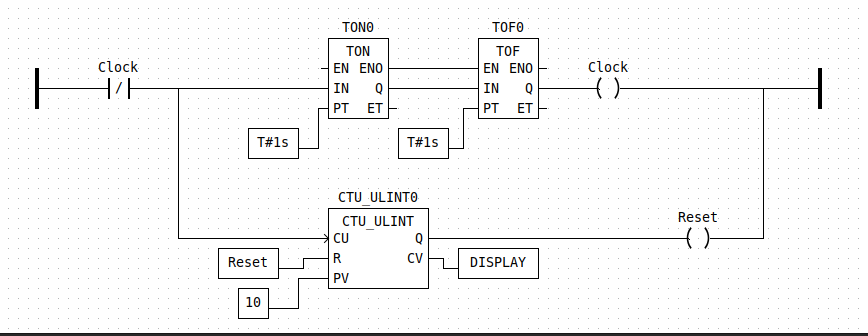
\includegraphics[width=0.8\textwidth]{images/clock.png}
    \caption{Clock}
    \label{fig:clock}
\end{figure}

\section{Extrator de Digitos}
O extrator de digitos foi implementado para separar os digitos do numero aleatório gerado, para que cada digito possa ser comparado com o botao pressionado pela vitima.

\begin{figure}[H]
    \centering
    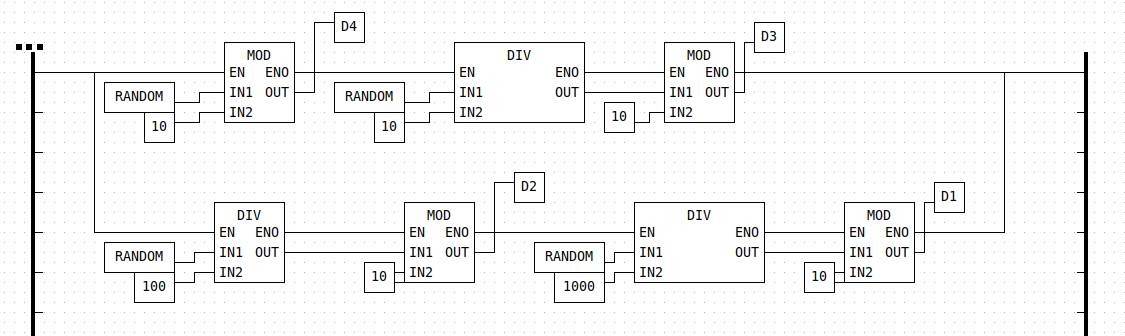
\includegraphics[width=0.8\textwidth]{images/digit_extractor.png}
    \caption{Extrator de Digitos}
    \label{fig:extrator_de_digitos}
\end{figure}

\section{Gerador de Numero Aleatório}
Para se gerar o numero aleatorio utilizou-se do Hull-Dobell Linear Congruential Generator definido por:

\begin{equation}
X_{(n+1)} = (aX_n + c)mod m
\end{equation}

Onde:
\begin{itemize} 
  \item m > 0
  \item 0 < a < m
  \item 0 <= c < m
  \item 0 <= X < m
  \item m potencia de 2, aki $ m = 2^{32} $
  \item a-1 divisivel por todos fatores primos de m, ou seja apenas divisivel por 2
  \item c diferente de 0
  \item m e c sao coprimos, c impar entao automaticamente coprimo de m
\end{itemize}

Para esse LCG utilizou-se os seguintes valores:
\begin{equation}
   a = 32310901
   c = 32310901
   m = 4294967296
\end{equation}

Deve gerar um Random quando a armadilha for ativada pela primeira vez e sempre que a Vitima cometer um erro. Como O perido aki seria de m, tira-se o modulo por 10000 para ter-se numeros entre 0-9999

\begin{figure}[H]
    \centering
    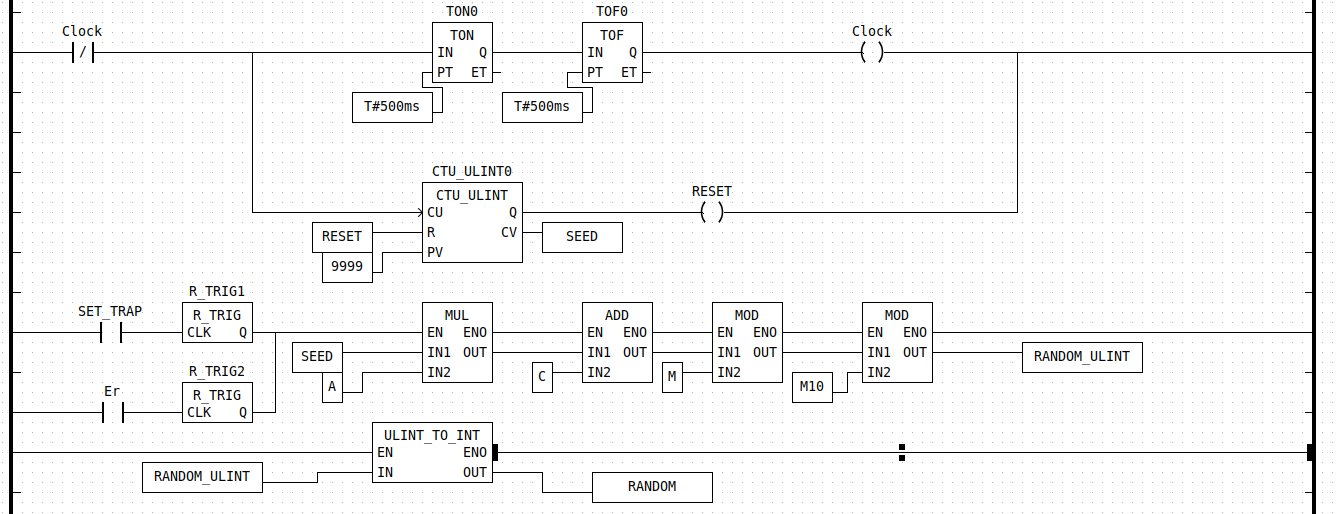
\includegraphics[width=0.8\textwidth]{images/random_generator.png}
    \caption{Gerador de Numero Aleatório}
    \label{fig:gerador_de_numero_aleatorio}
\end{figure}

\section{Temporizador}
Toda Vez que um erro ocorre (Er) deve-se remover 10s do Temporizador. Note que o programa usa um cronometro para se chegar ao tempo inbutido atraves das variaveis de entrada para minutos e segundos, porem o display exibe os valores como um temporizador. Para isso, o tempo total e convertido em um unico TIMER e depois manipulado para ser exibido como um temporizador.
A conversao para um TIMER total impede que se tenha valores negativos para segundos com a subtração por erro.
Ah mais não vai fica abaixo de zero quando ele erra os segundos forem menores que 10?
Não por que a conversao trabalha com o total em segundos e depois realizar a reconversao para minutos e segundos quand for exibir no display

\begin{figure}[H]
    \centering
    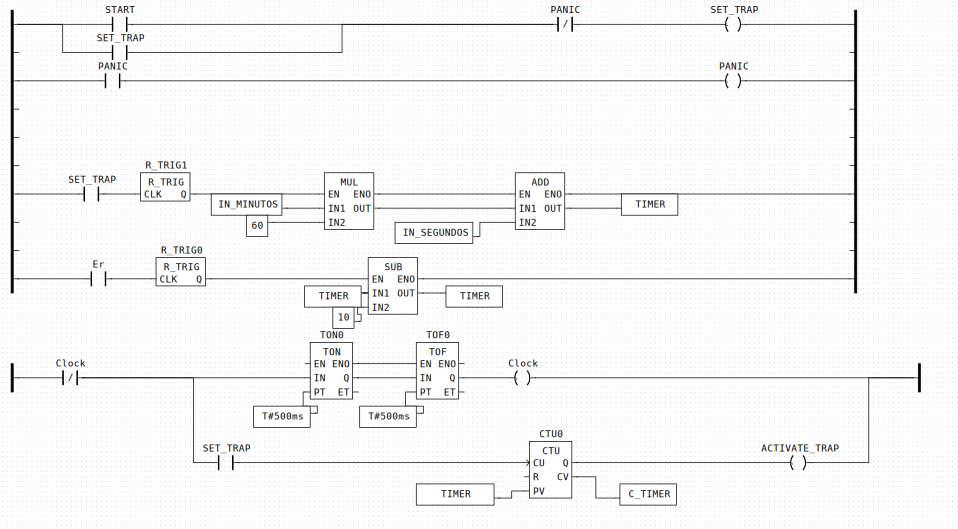
\includegraphics[width=0.8\textwidth]{images/sub_timer.png}
    \caption{Temporizador}
    \label{fig:temporizador}
\end{figure}

O Display converte o valor do TIMER, que é um cronometro, para o formato de um temporizador através de operações matematicas simples.

\begin{figure}[H]
    \centering
    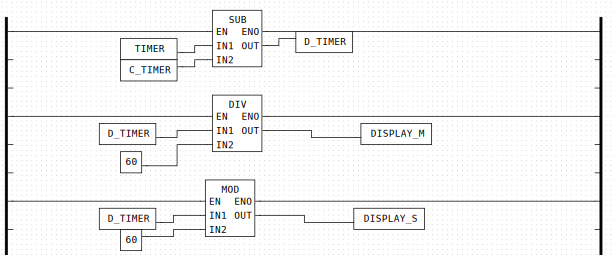
\includegraphics[width=0.8\textwidth]{images/display.png}
    \caption{Display do Temporizador}
    \label{fig:display_do_temporizador}
\end{figure}


\section{Botões}
Os botões são implementados como entradas digitais, e cada botão corresponde a um número de 1 a 4. Quando um botão é pressionado, o sistema verifica se o número do botão corresponde ao dígito atual do puzzle que a vítima deve pressionar. 
A seguinte imagem representa a implementação do botão 1, os outros botões são implementados de forma semelhante.

\begin{figure}[H]
    \centering
    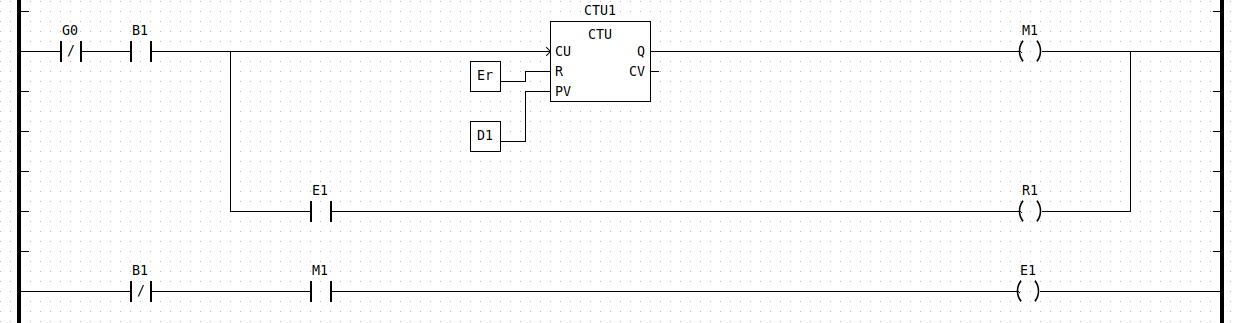
\includegraphics[width=0.8\textwidth]{images/button_input.png}
    \caption{Botão 1}
    \label{fig:botao_1}
\end{figure}

\subsection{Guarda de Pressionamento}
Guarda para garantir que não há mais de um botao sendo pressionado ao mesmo tempo
Usar combinacao de 4 em 2 = 6, de 4 em 3 = 4 e de 4 em 4 = 1 atraves da formula:
\begin{equation}
  c = \frac{n!}{r!(n-r)!}
\end{equation}

\begin{figure}[H]
    \centering
    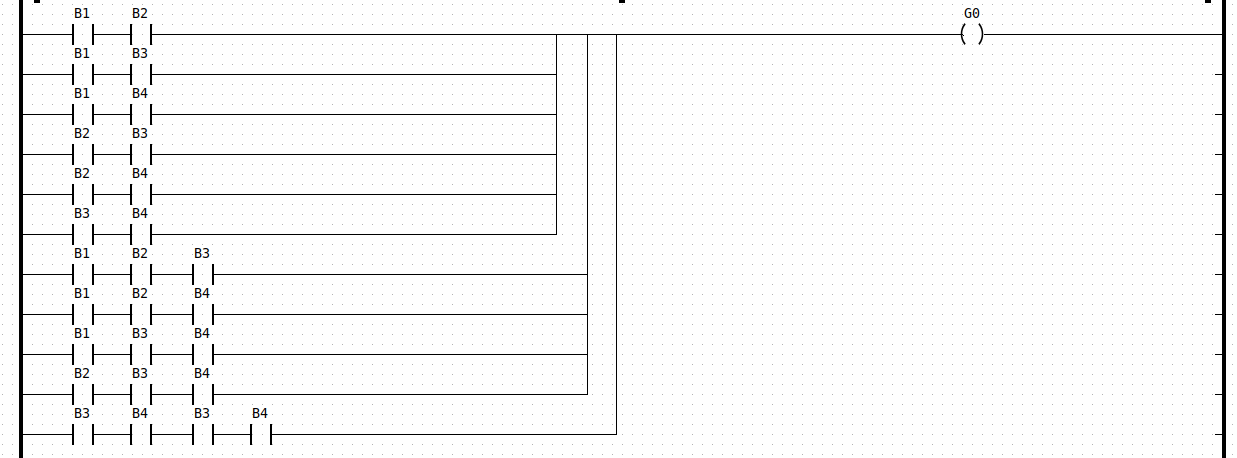
\includegraphics[width=0.8\textwidth]{images/button_guard.png}
    \caption{Guarda de Pressionamento}
    \label{fig:guarda_de_pressionamento}
\end{figure}

\subsection{Guarda de Valor}
Qualquer valor 0 em um dos digitos automaticamente ativa a memoria correspondente, independentemente da ordem. Por isso deve-se guardar a logica das outras memorias quand uma delas esta sempre ativa, não ativar erro de ordem quando uma delas é sempre positiva

\begin{figure}[H]
    \centering
    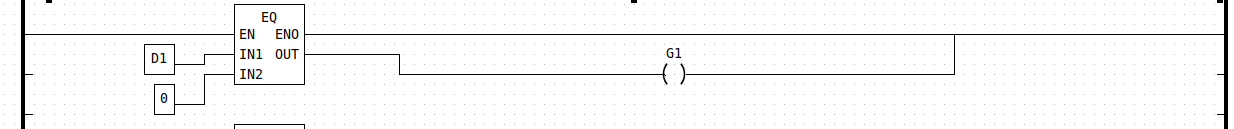
\includegraphics[width=0.8\textwidth]{images/button_value_guard.png}
    \caption{Guarda de Valor}
    \label{fig:guarda_de_valor}
\end{figure}

\subsection{Casos de Ordem}
A cada botao pressionado, deve-se verificar se o botao pressionado é o correto.

\begin{figure}[H]
    \centering
    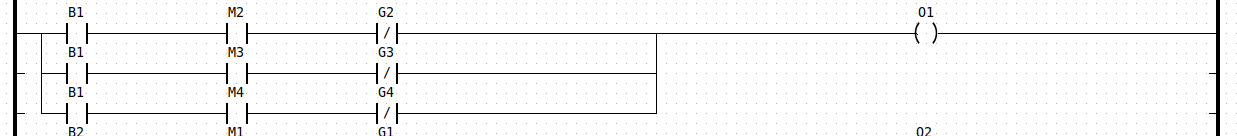
\includegraphics[width=0.8\textwidth]{images/button_order_case.png}
    \caption{Casos de Ordem}
    \label{fig:casos_de_ordem}
\end{figure}

\chapter{Conclusão}

O projeto construiu um sistema automatizado para simular uma armadillha onde a vitima se encontra amarrada em uma cadeira com a reverse bear trap presa em sua cabeça e precisa resolver o puzzle para se libertar. O sistema aplica conceitos de automatização para criar uma paródia em relação aos filmes da franquia \textit{Saw}, onde pode-se perceber claramente a necessidade de automatização para o funcionamento das armadilhas.


%%%%%%%%%%%%%%%%%%%%%%%%%%%%%%%%%%%%%%%%%%%%%%%%%%%%%%%%%%%%%%%%%%%%%%%%%%%%%%%%%
%% Source defintions
%%%%%%%%%%%%%%%%%%%%%%%%%%%%%%%%%%%%%%%%%%%%%%%%%%%%%%%%%%%%%%%%%%%%%%%%%%%%%%%%%
% When no use outcomment
%\include{base/sources}
%%%%%%%%%%%%%%%%%%%%%%%%%%%%%%%%%%%%%%%%%%%%%%%%%%%%%%%%%%%%%%%%%%%%%%%%%%%%%%%%%
%% Inserting the appendix
%%%%%%%%%%%%%%%%%%%%%%%%%%%%%%%%%%%%%%%%%%%%%%%%%%%%%%%%%%%%%%%%%%%%%%%%%%%%%%%%%
% When no use outcomment
\newpage
\appendix

\addcontentsline{toc}{chapter}{Apêndice}

\chapter{Bibliografia}

\end{document}
